% \documentclass[12pt]{article}

%%v helpful MIT exam schema, see http://www-math.mit.edu/~psh/exam/examdoc.pdf
 \documentclass[12pt]{exam} 
% \qformat{\textbf{Question \thequestion}\quad \thepoints\hfill } % Large depth to make space}
 \renewcommand{\thesubpart}{(\roman{subpart})}
 \renewcommand{\subpartlabel}{\thesubpart}
% \footer{}{}{Page \thepage\ de \numpages}
\addpoints
\pointsinmargin
% \boxedpoints
\renewcommand{\questionshook}{\setlength{\itemsep}{4mm}}
\renewcommand{\partshook}{
	\setlength{\itemsep}{0.2cm}
    	\setlength{\leftmargin}{-5pt}%
}

\usepackage{cmbright}

\pagestyle{empty} %for handouts
\addtolength{\jot}{2em} % this makes all formulae a bit more spaced vertically for handouts
\setlength{\parindent}{0pt} %we're not writing a novel
\renewcommand{\arraystretch}{1.5} %makes tables taller, so easier to write in

\usepackage[fleqn]{amsmath}
\usepackage{amssymb} %standard classy maths symbols
\usepackage[a4paper, margin=1in]{geometry} %makes it easy to specify where to put stuff on the page

\usepackage{siunitx} %v handy way of getting SI units to typeset correctly...
% \sisetup{locale = FR} %... and now it will use a comma for decimals

\usepackage[utf8]{inputenc}

% \usepackage[french]{babel} % frenchify everything (e.g. a Table becomes a Tableau)
% \usepackage{lmodern} % font with nicer French characters than standard
% \usepackage{textcomp} % and more help for special characters

\usepackage{tcolorbox} % basic but good package for boxes around text
\tcbset{colback=black!5!white}
% \usepackage{color} % colours
%\newcommand{\fillin}{\color{black!1!white}} %makes the text disappear
%\definecolor{fillin}{rgb} {1.00,1.00,1.00}
%\renewcommand{\fillin}{\color{blue}} \definecolor{fillin}{rgb} {0.00,0.00,1.00} %makes the filling in text appear (in blue)

\usepackage{enumitem} % can change the labels on lists, items, enumerates
\usepackage{setspace}

\usepackage{tikz} % interval diagrams, sets, etc.
%\usetikzlibrary{calc,trees,positioning,arrows,fit,shapes}
\usetikzlibrary{arrows.meta}

% Use a 'closing' sqrt symbol
\usepackage{letltxmacro}
\makeatletter
\let\oldr@@t\r@@t
\def\r@@t#1#2{%
\setbox0=\hbox{$\oldr@@t#1{#2\,}$}\dimen0=\ht0
\advance\dimen0-0.2\ht0
\setbox2=\hbox{\vrule height\ht0 depth -\dimen0}%
{\box0\lower0.4pt\box2}}
\LetLtxMacro{\oldsqrt}{\sqrt}
\renewcommand*{\sqrt}[2][\ ]{\oldsqrt[#1]{#2}}
\makeatother

\begin{document}

\textbf{Name:} \dotfill

\

\large
\begin{questions}


\question[6] Complétez le tableau.

\begin{tabular}{|c|c|c|}
\hline
Notation d’intervalle & Représentation graphique & Sous forme d’inégalité \\ \hline                  &   \begin{tikzpicture}


\draw[white] (0,0.8) -- (0.1,0.8);
\draw[thick, ->] (0,0) -- (6,0);
\draw[white] (0,-0.8) -- (0.1,-0.8);

\end{tikzpicture}                           & $6 < x \leq 7$   \\ \hline
$x \in \, ]\!- \!\infty; \, 4[$   & \begin{tikzpicture}


\draw[white] (0,0.8) -- (0.1,0.8);
\draw[thick, ->] (0,0) -- (6,0);
\draw[white] (0,-0.8) -- (0.1,-0.8);

\end{tikzpicture}                          &                  \\ \hline
                  & 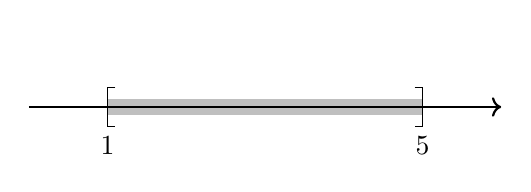
\begin{tikzpicture}


\draw[white] (0,1) -- (0.1,1);
\fill[white!50!gray] (1,-0.1) rectangle (5,0.1);
\draw[thick, ->] (0,0) -- (6,0);
\draw (1.1,0.25) -- (1,0.25) -- (1,-0.25) node[below] {1} -- (1.1, -0.25);
\draw (4.9,0.25) -- (5,0.25) -- (5,-0.25) node[below] {5}  -- (4.9, -0.25);

\end{tikzpicture}                       &                  \\ \hline
\end{tabular}



\question[4] Study the function $f$.

\vspace{3mm}
\begin{parts}

\begin{minipage}[t]{0.55\textwidth}
\part Explain why $f$ is a function.
\fillwithdottedlines{14mm}

\part What is the image of 1 by $f$?
\fillwithdottedlines{9mm}

\end{minipage}
\hspace{5mm}
\begin{minipage}[t]{0.4\textwidth}
\vspace{-8mm}
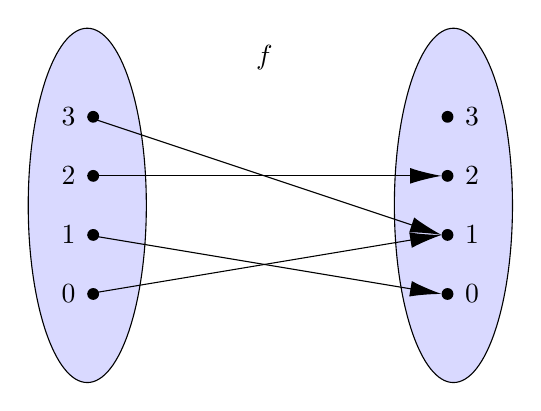
\begin{tikzpicture}[scale=0.75]

\draw[fill=blue!15] (0,1.5) ellipse (1cm and 3cm); 
\foreach \x in {0, 1, 2, 3}{
\fill (0.1, \x) circle (1mm) node[left=1mm] {$\x$};
}


\draw[fill=blue!15] (6.2,1.5) ellipse (1cm and 3cm); 
\foreach \x in {0, 1, 2, 3}{
\fill (6.1, \x) circle (1mm) node[right=1mm] {$\x$};
}

\draw[-{Latex[length=4mm,width=2mm]}] (0,0)--(6,1);
\draw[-{Latex[length=4mm,width=2mm]}] (0,1)--(6,0);
\draw[-{Latex[length=4mm,width=2mm]}] (0,2)--(6,2);
\draw[-{Latex[length=4mm,width=2mm]}] (0,3)--(6,1);

\node at (3, 4) {$f$};
\end{tikzpicture}
\end{minipage}

\part What are the pre-images of 1 by $f$?
\fillwithdottedlines{9mm}

\part Work out $f(f(3))$
\fillwithdottedlines{8mm}
\end{parts}


\vfill



\question \textbf{Bonus.} If $f^{n+1}(x) = f \big(f^n(x)\big)$ and $f^1(x)=f(x)$, what is $f^{2023}(1)$?

\end{questions}

\begin{tcolorbox}

\textbf{Name of marker:}

\begin{center}
\gradetable[h][questions]
\end{center}

\end{tcolorbox}

\end{document}